\documentclass[11pt, a4paper, twoside]{article}   	% use "amsart" instead of "article" for AMSLaTeX format

\usepackage{geometry}                		% See geometry.pdf to learn the layout options. There are lots.
\usepackage{pdfpages}
\usepackage{caption}
\usepackage{minted}
\usepackage[german]{babel}			% this end the next are needed for german umlaute
\usepackage[utf8]{inputenc}
\usepackage{color}
\usepackage{graphicx}
\usepackage{titlesec}
\usepackage{fancyhdr}
\usepackage{lastpage}
\usepackage{hyperref}
% http://www.artofproblemsolving.com/wiki/index.php/LaTeX:Symbols#Operators
% =============================================
% Layout & Colors
% =============================================
\geometry{
   a4paper,
   total={210mm,297mm},
   left=20mm,
   right=20mm,
   top=20mm,
   bottom=30mm
 }	

\definecolor{myred}{rgb}{0.7,0.3,0.4}
\definecolor{mygreen}{rgb}{0,0.6,0}
\definecolor{mygray}{rgb}{0.5,0.5,0.5}
\definecolor{mymauve}{rgb}{0.58,0,0.82}

\setcounter{secnumdepth}{4}


% the default java directory structure and the main packages
\newcommand{\dotNetRoot}{../source/dot-net}
\newcommand{\javaRoot}{../source/java}
\newcommand{\imagesRoot}{images}
% the default subsection headers
\newcommand{\ideaSection}{Lösungsidee}
\newcommand{\sourceSection}{Source-Code}
\newcommand{\testSection}{Tests}

% =============================================
% Code Settings
% =============================================
\newenvironment{code}{\captionsetup{type=listing}}{}
\newmintedfile[javaSourceFile]{java}{
	linenos=true, 
	frame=single, 
	breaklines=true, 
	tabsize=2,
	numbersep=5pt,
	xleftmargin=10pt,
	baselinestretch=1,
	fontsize=\footnotesize
}
\newmintinline[inlineJava]{java}{}
\newminted[javaSource]{java}{
	breaklines=true, 
	tabsize=2,
	autogobble=true,
	breakautoindent=false
}
\newmintedfile[xmlSourceFile]{xml}{
	linenos=true, 
	frame=single, 
	breaklines=true, 
	tabsize=2,
	numbersep=5pt,
	xleftmargin=10pt,
	baselinestretch=1,
	fontsize=\footnotesize
}
\newmintedfile[propertiesFile]{properties}{
	linenos=true, 
	frame=single, 
	breaklines=true, 
	tabsize=2,
	numbersep=5pt,
	xleftmargin=10pt,
	baselinestretch=1,
	fontsize=\footnotesize
}
% =============================================
% Page Style, Footers & Headers, Title
% =============================================
\title{Übung 3}
\author{Thomas Herzog}

\lhead{Übung 3}
\chead{}
\rhead{
\includegraphics[scale=0.10]{FHO_Logo_Students.jpg}}

\lfoot{S1310307011}
\cfoot{}
\rfoot{ \thepage / \pageref{LastPage} }
\renewcommand{\footrulewidth}{0.4pt}
% =============================================
% D O C U M E N T     C O N T E N T
% =============================================
\pagestyle{fancy}
\begin{document}
\setlength{\headheight}{15mm}
%\includepdf[pages={1-3}]{Swe4xA05-BB.pdf}
{\color{myred}
	\section
		{UFO (Ultimate - Festival - Organizer)}
}
Folgende Dokumentation stellt die Gesamtdokumentation der aufbauenden Übung UFO dar, die im Zuge der Realisierung iterativ über die drei Ausbaustufen hinweg erweitert wird. \\

\subsection{Ausbaustufe 1 (ADO.NET)}
Folgender Teil dokumentiert die erste Ausbaustufe der aufbauenden Übung UFO. In diesem Teil wird die Persistenz Schicht in .NET unter Hilfenahme von ADO.NET implementiert. Aufgrund der Analyse der Gesamtaufgabenstellung wurde entschieden das vorerst nur die Persistenz Schicht an sich, also INSERT, UPDATE, DELETE der einzelnen Entitäten realisiert wird, da die Geschäftslogik erst bei der Realisierung der Administration und des Webzugriffs endgültig feststehen wird. \\\\
Im Zuge der Realisierung des Webzugriffs wird auch der Web-Service implementiert werden müssen, der die Daten der Web Applikation zur Verfügung stellt. Dieser soll die Daten bereits gefiltert und strukturiert zur Verfügung stellen, daher besteht eine gewisse Abhängigkeit zwischen dem Web-Service und der Web Applikation sowie auch der Client Administration.\\\\
Daher werden die Web-Service Implementierung und die Administration die eigentliche Geschäftslogik enthalten, die 
in einer Transaktion abgearbeitet und im wesentlichen aus den logischen Prüfungen gegen die Datenbank bestehen wird sowie der Speicherung und Löschung von Entitäten über die Administration. Die einzelnen Datenabfragen, die benötigt werden können einfach hinzugefügt werden.

\subsubsection{Systemaufbau}
Folgend ist der Systemaufbau der Persistenz Schicht dokumentiert.\\\\
Die folgende Auflistung illustriert die Projektstruktur der Persistenz Schicht:
\begin{enumerate}
	\item\emph{UFO.Server.Data.Api}\\
	 Dieses Projekt enthält die Spezifikation der Persistenz Schicht in Form von 	      Interfaces, abstrakten Klassen, Exceptions und den Entitäten, die wie bei einem ORM-Mapper DB unabhängig sein sollen (sofern möglich).
	 \item\emph{UFO.Server.Data.MySql}\\
	 Dieses Projekt enthält die MySql spezifische Implementierung der Persistenz Schicht.
	 \item\emph{UFO.Server.Test.Data.MySql}\\
	 Dieses Projekt enthält die MySql spezifischen Tests der Persistenz Schicht.
	 \item\emph{UFO.Common.Util}\\
	 Dieses Projekt enthält die Utlities für die UFO Infrastruktur in .NET, die nicht spezifisch einen Systemteil zuzuordnen sind.
	 \item\emph{ufo-data-generator}\\
	 Ein kleines Java Projekt welches eine Java Main Klasse enthält und die benötigen Ressourcen um das Testdatenskript zu erstellen. Hierzu wurde \emph{freemarker} verwendet.
\end{enumerate}
Alle .NET Systemteile werden unter dem Namensraum \emph{UFO.*} zusammengefasst.

\newpage
Die folgende Auflistung illustriert die verwendeten Technologien und Frameworks:
\begin{enumerate}
	\item\emph{MySql}\\
	Es wird eine MySql Datenbank verwendet, die Open-Source ist und eine Integration in .NET besitzt.
	\item\emph{NUNIT}\\
	Als Test-Framework wird NUNIT verwendet, da es mehr Funktionalität mitbringt als das Standard Test-Framework integriert in .NET.
	\item\emph{ADO.NET}\\
	Als Persistenz Provider wird wie gewünnscht ADO.NET und kein ORM Mapper verwendet.
	\item\emph{freemarker}\\
	Template-Engine in Java mit der das Testdaten SQL Skript erstellt wird.
\end{enumerate}

\newpage
\subsubsection{Datenbank}
Es wurde als Datenbank MySql und Moderlierungstool MySql Workbench gewählt, da diese Datenbank erstens Open-Source, zweitens eine gute .NET Integration vorhanden ist sowie drittens bereits Erfahrungen mit dieser Datenbank vorhanden waren.\\\\
Es wurden folgende Skripten generiert die einerseits für die Tests und andererseits für die Generierung der Testdaten genutzt werden. Diese Skripten befinden sich im Projekt \emph{UFO.Server.Data.MySql/Resources}.\\
\begin{enumerate}
	\item\emph{createDatabase.sql}\\
	Ein vollständiges Skript für das Anlegen der Datenbank mit allen Constraints und verwendeten Triggern.
	\item\emph{deleteDatabase.sql}\\
	Ein Skript welches alle Einträge in der Datenbank löscht.
	\item\emph{dropDatabase.sql}\\
	Ein Skript für das Droppen der Datenbank UFO.
	\item\emph{createTestData.sql}\\
	Ein Skript welches die Testdaten generiert.
\end{enumerate}
\ \\
Die Testdaten wurden mit einer Java Applikation mit Hilfe von \emph{Freemarker} erstellt, welches eine Template Engine darstellt. Die Daten werden von \emph{*.csv} Dateien zur Verfügung gestellt und anschließend über eine Java Konsolen Applikation verarbeitet. Diese Applikation liest die Daten ein, verpackt diese in Pojos, generiert dynamische Daten, wie z.B.: die Aufführungen mit den Aufführungszeiten und stellt diese Daten einem Template zur Verfügung.

\newpage
Das folgende ER-Diagramm illustriert das implementierte Datenbank Schema.
\begin{figure}[h]
	\centering
	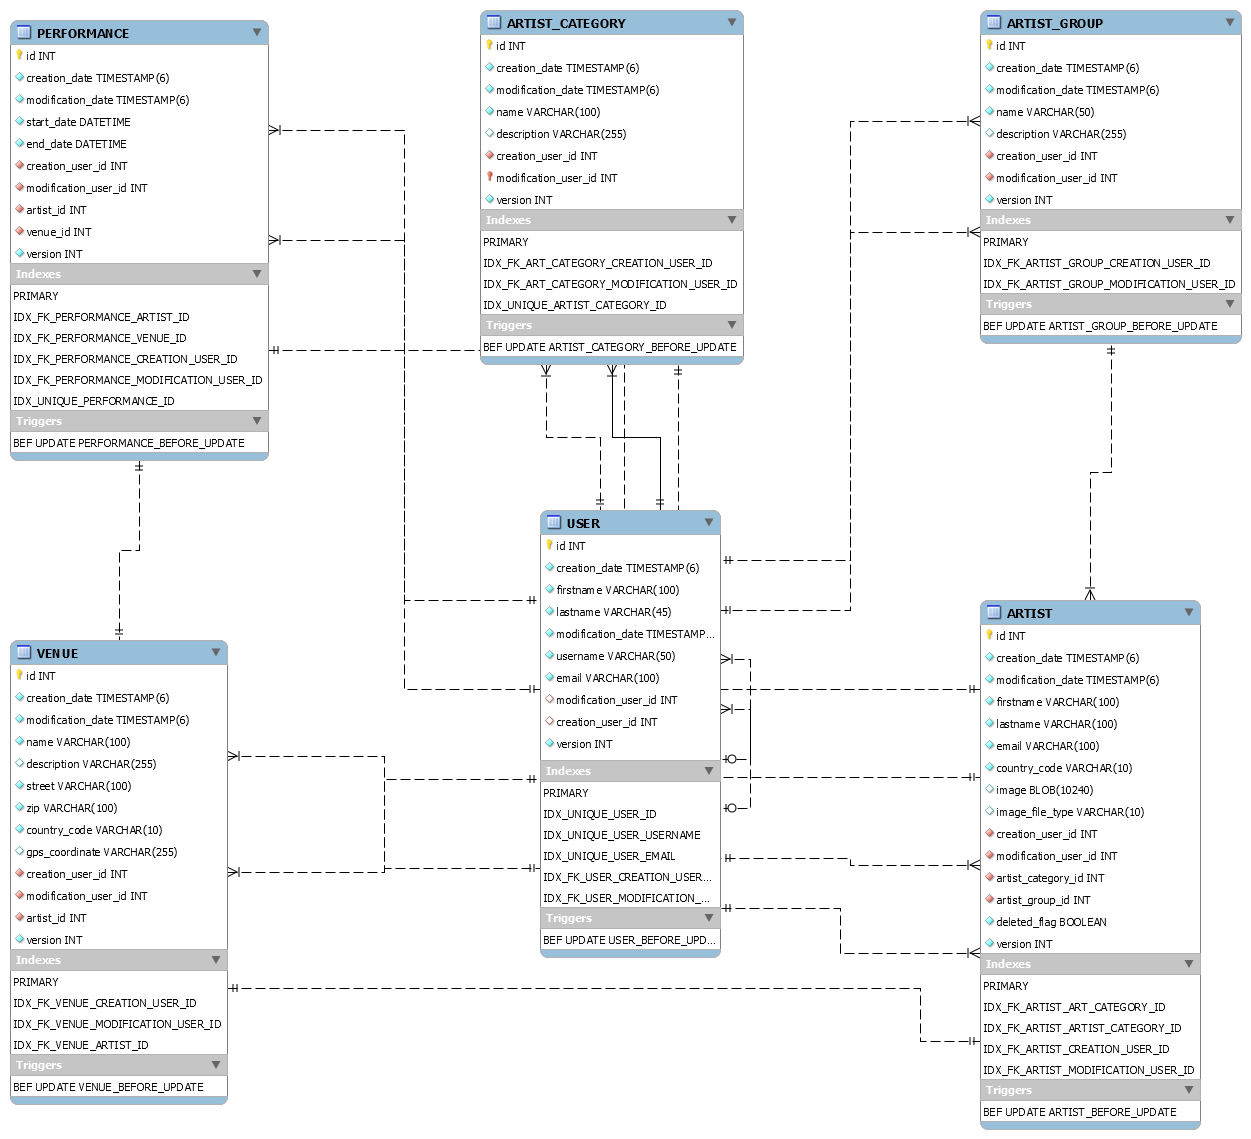
\includegraphics[scale=0.35]{\imagesRoot/er_diagram.PNG}
	\caption
	{ER-Diagramm des Schema 'UFO'}
\end{figure}
\ \\
Auf jeder Entität wurde eine Spalte für die Versionierung eingeführt (MySqlDbType.LONG), die über einen Update-Trigger bei jedem Update um eins erhöht wird sowie auch das Modifizierungsdatum. Ein ganzzahliger Datentyp erschient hier mehr sinnvoll, da es hier mit Sicherheit keine Kollisionen geben kann, nicht so wie bei einem Zeit Datentyp.\\\\
Ebenso halten alle Entitäten eine Referenz auf den Benutzer der Sie erstellt sowie zuletzt modifiziert hat. Dies dient der Nachverfolgbarkeit von Änderungen, zumindest wer zuletzt eine Änderung vorgenommen hat.

\newpage
\subsubsection{Klassenhierarchien}
Folgend sind die Klassenhierarchien der implementierten Klassen und Interfaces dokumentiert.\\

\textbf{\emph{IDao}}\\
Folgendes Klassendiagramm zeigt die Hierarchie des Interfaces \emph{IDao}, das der Basistyp für alle implementierten DAO Interfaces dient, da es bereits alle Basisaktionen auf eine Entität definiert.
\begin{figure}[h]
	\centering
	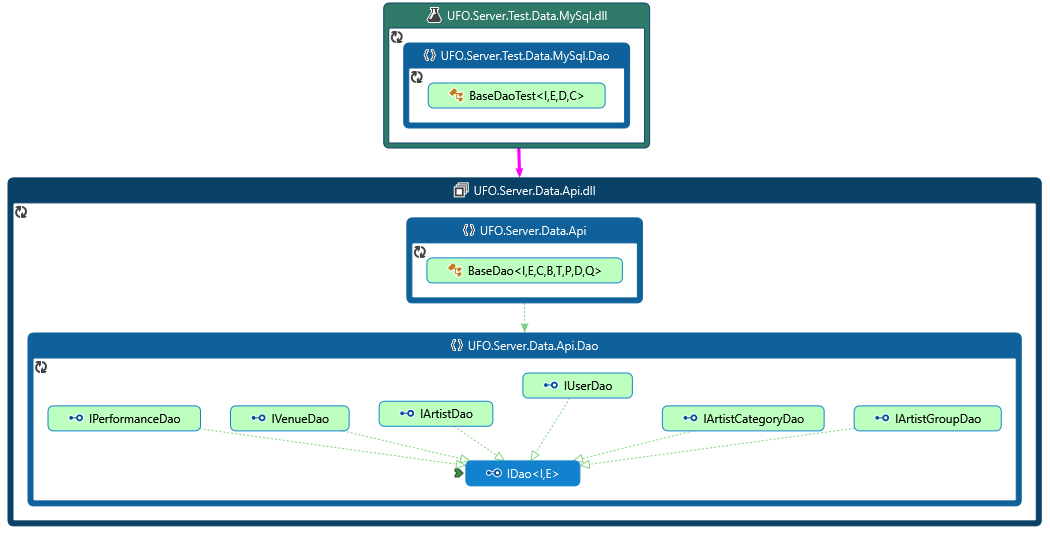
\includegraphics[scale=1]{\imagesRoot/idao_map.PNG}
	\caption
	{Klassenhierarchie IDao Interface}
\end{figure}
\ \\
Die Basisklasse  \emph{BaseDao} implementiert alle Methoden, die in \emph{IDao} definiert wurden für alle implementieren Entitäten sofern sie \emph{IEntity} implementieren. Dieser generische und abstrakte Ansatz erlaubt es dass die Basisfunktionalität eines DAOs nur einmal für alle Entitätstypen, die \emph{IEntity} implementieren, implementiert werden musste.\\\\
Die \emph{DAOs} für die einzelnen Entitäten werden zukünftig Methoden implementieren, die spezifische Datenbankabfragen realisieren, die z.B.: eine komplexe \emph{where caluse} aufweisen, die ihrerseits wieder einen Teil der Geschäftslogik enthält, welche noch nicht vollständig bekannt ist.

\newpage
\textbf{\emph{IEntity}}\\
Folgendes Klassendiagramm illustriert die Klassenhierarchie des Interfaces \emph{IEntity}, welches den Basistyp für alle Entitäten darstellt.
\begin{figure}[h]
	\centering
	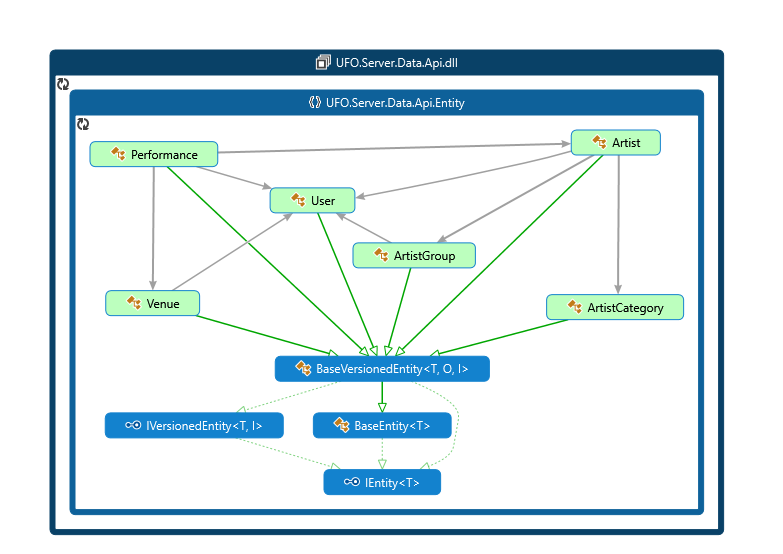
\includegraphics[scale=1]{\imagesRoot/ientity_map.PNG}
	\caption
	{Klassenhierarchie IEntity Interface}
\end{figure}
\ \\
Es wurden Basisentitäten eingeführt, welche eine Basisstruktur definieren dies sich Entitäten unterwerfen müssen wenn sie von diesen Klassen ableiten. Somit wird eine konsistente Struktur der Entitäten bzw. deren Tabellenrepräsentation gewährleistet.\\\\
Die Aufteilung von \emph{IEntity} und \emph{IVersionedEntity} wurde eingeführt, da eine Entität nicht zwangsweise versionierbar sein muss. Ebenso wurde mit den abstrakten Klassen verfahren, die jetzt eine Hierarchie abbilden anstatt die gesamte Funktionalität in eine abstrakte Klasse zu packen.

\newpage 
\textbf{\emph{IEntityHelper}}\\
Folgendes Klassendiagramm illustriert die Klassenhierarchie des Interfaces \emph{IEntityHelper} welches die Utility Methoden für das generieren von Entitäten definiert.
\begin{figure}[h]
	\centering
	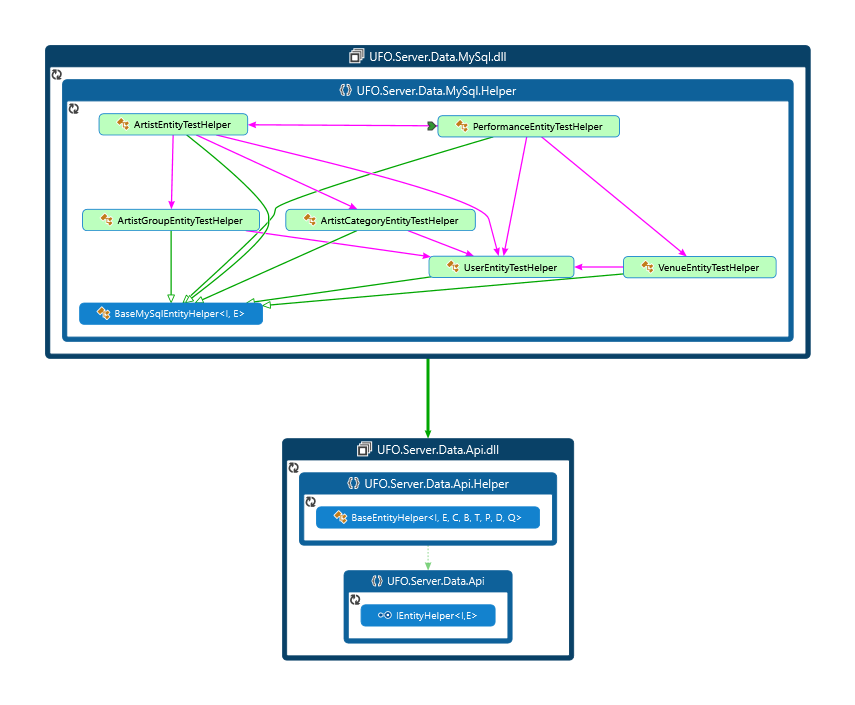
\includegraphics[scale=1]{\imagesRoot/ientityhelper_map.PNG}
	\caption
	{Klassenhierarchie IEntityHelper Interface}
\end{figure}
\ \\
Dieses Interface und dessen Implementierungen diesen als Hilfestellung für die Test und die Generierung von Testdaten über die Entitäten Modelle. Die abstrakte Basisklasse \emph{BaseEntityHelper} implementiert einige der Interface Methoden und stellt eine Persistenzprovider unabhängige Implementierung für das einfache Speichern von Entitäten zur Verfügung. Diese Hilfsklassen entstanden aufgrund der generischen Testklasse \emph{BaseDaoTest}, die die Entitäten nicht erzeugen kann und daher diese von außen zur Verfügung gestellt werden müssen.

\newpage
\textbf{\emph{BaseCommandBuilder}}\\
Folgendes Klassendiagramm illustriert die abstrakte Klasse \emph{BaseCommandBuilder} die das Handling mit einen \emph{DbCommand} beinhaltet. 
\begin{figure}[h]
	\centering
	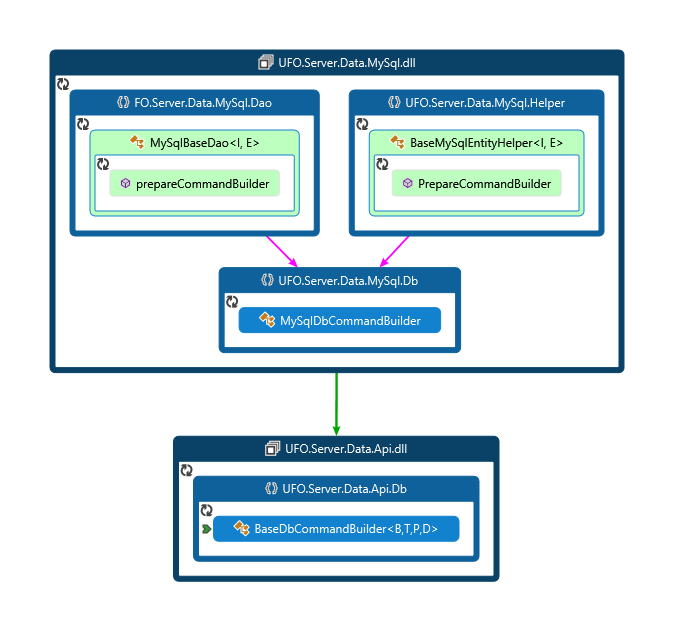
\includegraphics[scale=1]{\imagesRoot/basecommandbuilder_map.PNG}
	\caption
	{Klassenhierarchie der abstrakte Klasse BaseCommandBuilder}
\end{figure}
\ \\
Um zu vermeiden sich mit dem Code des Erstellens, Modifizierens und Verwerfens eines \emph{DbCommand}, in unserem Fall ein \emph{MySqlDbCommand}, herumschlagen zu müssen, wurde beschlossen eine Hilfsklasse einzuführen, die uns dieses Handling mit einem \emph{DbCommand} abnimmt.
Da sich hier eine Fluent-API gut anwenden lässt, wurde diese Funktionalität in Form eines Builder abgebildet.

\newpage
\textbf{\emph{IQueryCreator}}\\
Folgendes Klassendiagramm illustriert das Interface \emph{IQueryCreator}, die die Datenbank spezifischen Statements enthält.
\begin{figure}[h]
	\centering
	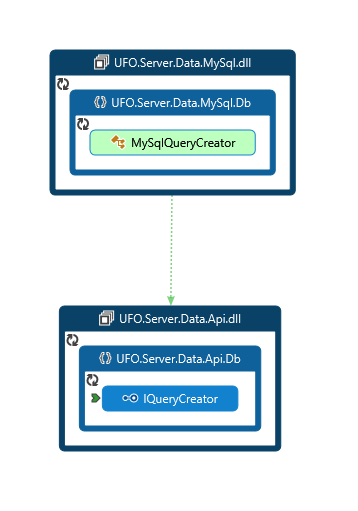
\includegraphics[scale=1]{\imagesRoot/iquerycreator_map.PNG}
	\caption
	{Klassenhierarchie des Interface \emph{IQueryCreator}}
\end{figure}
\ \\
Diese Interface abstrahiert die Datenbank spezifischen Statements von der Klient Logik. Ebenso erlaubt sie es alle Statements in einem Interface abzubilden und diese an einer Stelle pro Entität zu bündeln. 

\newpage
\subsubsection{Hilfsklassen}
Im folgenden werden die Hilfsklassen beschrieben, die eingeführt wurden um sich wiederholende und daher immer wiederkehrende Funktionalitäten zu kapseln und zentral zur Verfügung zu stellen.\\\\

\textbf{\emph{EntityMetamodel}}\\
Diese Klasse löst die Meta-Informationen eines \emph{IEntity} Typs auf und stellt diese aufbereitet nach außen zur Verfügung. Da sich diese Daten zur Laufzeit nicht ändern und daher nur einmalig erzeugt werden sollen, wird eine Factory \emph{EntityMetamodelFactory} eingeführt, die  das Caching der \emph{EntityMetamodel} übernimmt.\\\\

\textbf{\emph{EntityBuilder}}\\
Diese Klasse wurde eingeführt um die Transformation von den Entitäten zur Datenbank und visa versa zu unterstützen, wobei hier einerseits die Werte der Properties, die auf die Datenbank serialisierbar sind, ausgelesen und auf den Property gemapped werden und andererseits die De-Serialisierung vom \emph{IDataReader} zu einer Entität.\\\\

\textbf{\emph{IDbTypeResolver}}\\
Implementierungen dieses Interface lösen einen C\# Typ in einen korrespondierenden Datenbank spezifischen Typ auf.\\\\

\textbf{\emph{DbConnectionFactory}}\\\\
Diese Klasse erstellt und verwaltet die verwendeten \emph{DbConnection} Instanzen. Der Typ der zu verwendenden \emph{DbConnection} wird über die \emph{App.config} definiert, sowie der \emph{ConnectionString}.

\newpage
\subsubsection{Tests}
Die Tests bestehen aus einer einzigen Testklasse, die das \emph{IDao} Interface bzw. die dessen Ableitungen bzw. dessen Implementierungen, die zurzeit nur aus der Implementierung in \emph{BaseDao} bestehen. Also die Basis Dao Funktionalitäten beinhalten wie.\\
\begin{enumerate}
	\item\emph{dao.ById // Throws Exception}
	\item\emph{dao.Find // Returns null}
	\item\emph{dao.Update}
	\item\emph{dao.Persist}
	\item\emph{dao.Delete}
	\item\emph{dao.CheckIfExists}
\end{enumerate}
Die generische Testklasse \emph{BaseDaoTest}  wird mit \emph{NUNIT} Attributen versehen, die die Testklasse mit den zur Verfügung gestellten Typen instanzieren. Danach wird in der Setup Methode die verwendeten Ressourcen über Reflection instanziert und in der Tear-Down Methode disposed. Hier ist die Typinformation zur Laufzeit sehr Hilfreich. In Java als Beispiel würde hier dies Javas Type Erasure unmöglich machen.
\begin{figure}[h]
	\centering
	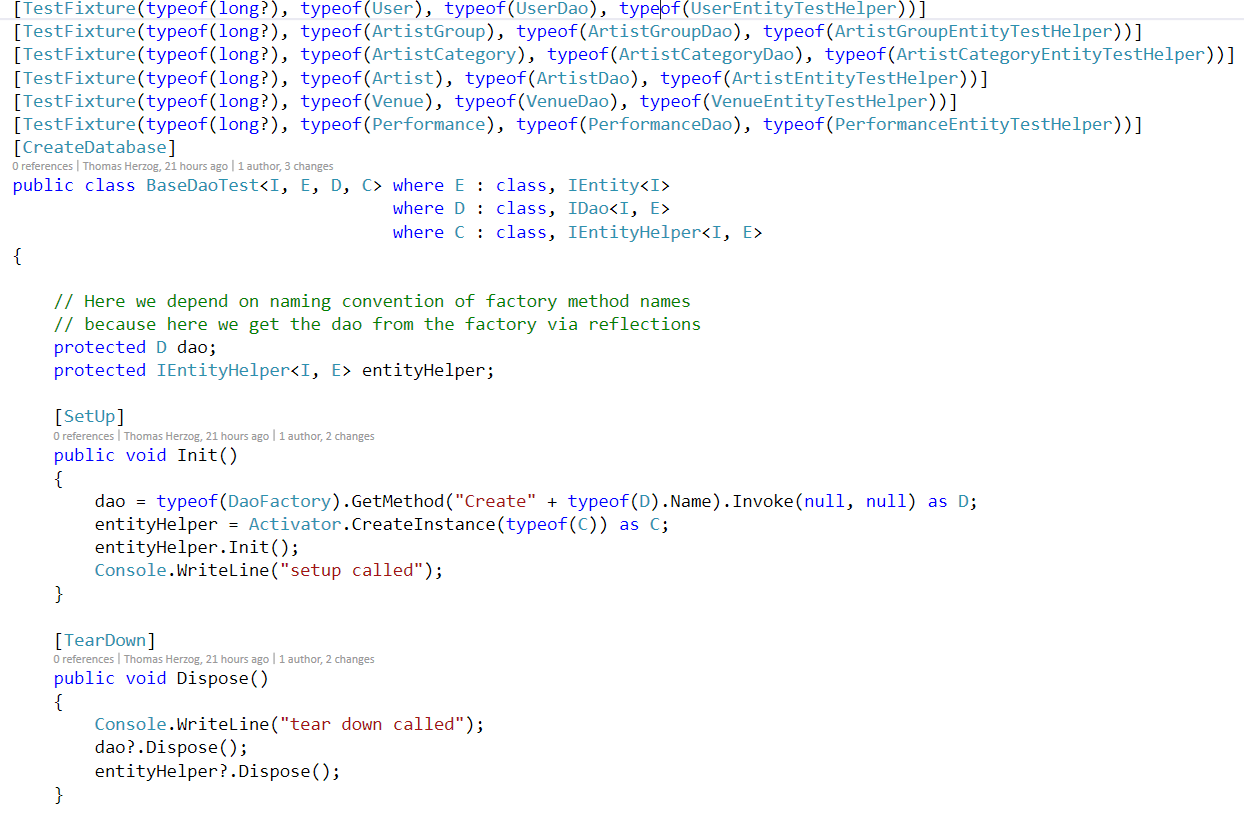
\includegraphics[scale=0.65]{\imagesRoot/basedaotest_screenshot.PNG}
	\caption
	{Ausschnitt aus der Testklasse \emph{BaseDaoTest}}
\end{figure}

\subsection{Ausbaustufe 2 (Commander)}
Folgender Teil dokumentiert die zweite Ausbaustufe des Projektes \emph{UFO} in dem die Administration mit WPF implementiert werden sollte.\\\\
Folgende Projekte wurden der Solution hinzugefügt.
\begin{enumerate}
	\item\emph{UFO.Commander.ServiceApi}\\
	Diese Projekt enthält die Schnittstellen Spezifikation für den Service Layer.
	\item\emph{UFO.Commander.Service.Impl}\\
	Dieses Projekt enthält die Implementierungen der Service Schnittstellen Spezifikationen
	\item\emph{UFO.Commander.Wpf.Administration}\\
	Dieses Projekt enthält die WPF Anwendung, die die Administration abbildet.
\end{enumerate}
\ \\
Des Weiteren wurde der Wurzelnamensraum auf \emph{UFO} beschränkt unter dem jetzt alle Projekte liegen.

\newpage
\subsubsection{Klassenhierarchien}
Folgender Teil der Dokumentation dokumentiert die definierten Klassenhierarchien der WPF Anwendung und des Service Layers.\\\\

\emph{\textbf{IService}}\\
Folgendes Klassendiagramm zeigt die Hierarchie des Interfaces \emph{IService}, welche die Wurzel aller Service Interfaces darstellt und \emph{IDisposable} erweitert. Somit ist jeder abgeleiteter Service dazu gezwungen die Methode \emph{Dispose} zu implementieren um dort seine gebundenen Ressourcen freizugeben. Des Weiteren wurde eine Basisklasse namens \emph{BaseService} eingeführt, welche die Datenbankverbindung und Transaktionsmethoden implementiert, sodass die abgeleitet Klassen diese Nutzen können.
\begin{figure}[h]
	\centering
	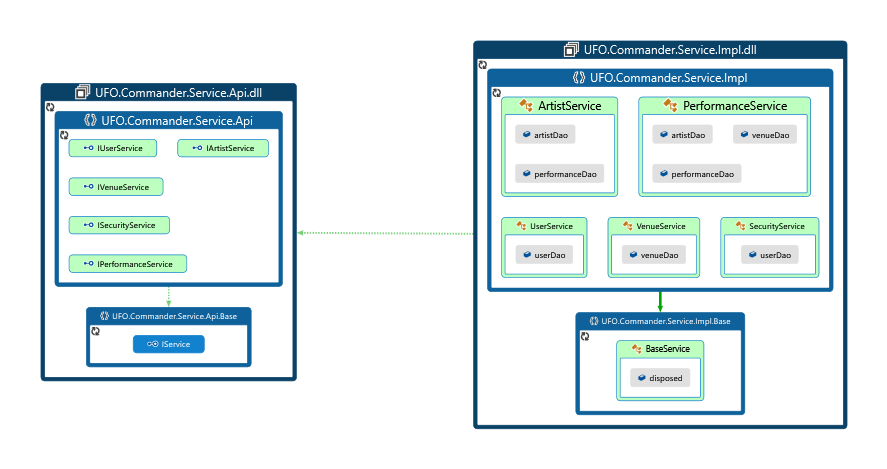
\includegraphics[scale=0.8]{\imagesRoot/iservice_map.PNG}
	\caption
	{Basis Interface für Service Interfaces und Implementierungen}
\end{figure}
\ \\
Alle Services bekommen in Ihrem Konstruktor eine \emph{DbConnection} Instanz übergeben, da alle verwendeten \emph{DAO} Implementierungen dieselbe Datenbank Verbindung nutzen müssen, damit alle sich in derselben Transaktion bewegen.

\newpage
\textbf{\emph{ITabModel}}\\
Folgendes Klassendiagramm zeigt die Hierarchien des Interfaces \emph{ITabModel}, die Operationen definiert, die von der Klasse \emph{TabController} verwendet werden. Die Klasse \emph{TabController} wurde eingeführt um \emph{ITabModel} Instanzen zu initialisieren und beim Wechseln eines Tab aufzuräumen.
\begin{figure}[h]
	\centering
	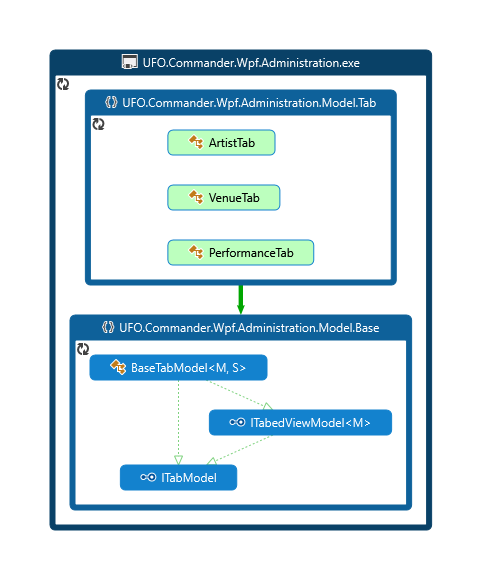
\includegraphics[scale=0.8]{\imagesRoot/basetabmodel_map.PNG}
	\caption
	{Basis Interface für Tab-Model Implementierungen}
\end{figure}
\ \\
Das Interface \emph{ITabedViewModel} definiert die Struktur der Implementierten Tab-Klassen, somit verhält sich jeder Tab gleichermaßen und kann beliebig erweitert werden, je nach seinem View-Content.

\newpage
\textbf{\emph{BasePropertyChangeViewModel}}\\
Folgendes Klassendiagramm zeigt die Hierarchien der Basisklasse \emph{BasePropertyChangeViewModel}, die die Wurzelklasse aller implementierten \emph{ViewModels} darstellt, da es immer mindesten einen Property gibt der diesen Event benötigt. Des Weiteren wurde die Klasse \emph{BaseValidationViewModel} eingeführt die die erste Ableitung von \emph{BasePropertyChangeViewModel} darstellt und die Logik für die Validierung über \emph{System.ComponentModel.DataAnnotations} realisiert. Von dieser Klasse erbt die Basisklasse \emph{BaseEntityViewModel}, die als Wrapper für ViewModels verwendet wird, die eine \emph{IEntity} Instanz für die View wrappen.
\begin{figure}[h]
	\centering
	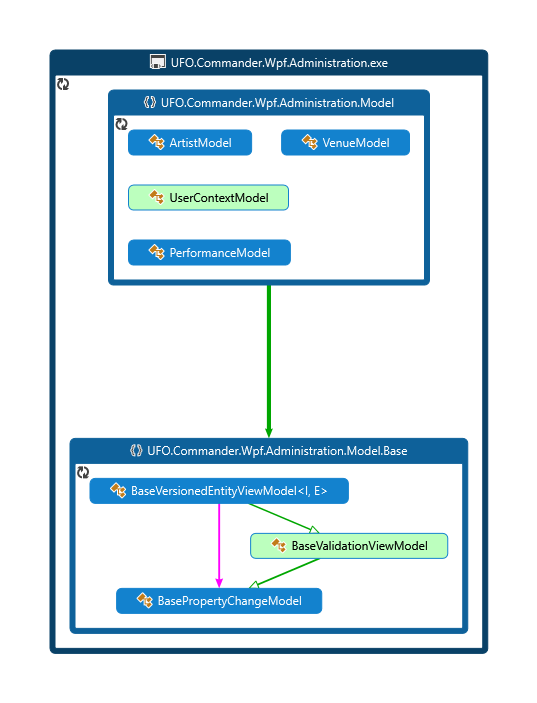
\includegraphics[scale=0.8]{\imagesRoot/viewmodelinheritance_map.PNG}
	\caption
	{Basisklasse für ViewModels}
\end{figure}
\ \\
Die Klasse \emph{UserContextModel} wurde eingeführt um einen eingeloggten Benutzer zu repräsentieren und wird als statischer Property der Klasse \emph{App} definiert, da es nur einen eingeloggten Benutzer pro gestarteter Anwendung geben kann. Alle Klassen, die auf den UserContext angewiesen sind müssen die Instanz der Klasse \emph{App} verwenden.

\newpage
\textbf{\emph{SimpleObjectModel}}\\
Folgendes Klassendiagramm zeigt die Hierarchien der Klasse \emph{SimpleObjectModel}, die eingeführt wurde um in Listen, Comboboxen und dergleichen Entitäten für die Darstellung zu halten. Die Controls verwenden Konverter, in denen aus der String Repräsentation wieder in die Entität konvertiert wird. Diese Klasse hält hierbei eine object Instanz (z.B.: Artist) und den anzuzeigenden Label. In den Konvertern wird eine Instanz \emph{SimpleObjectModel} aus dem zu verwaltenden Objekt erzeugt und visa versa.
\begin{figure}[h]
	\centering
	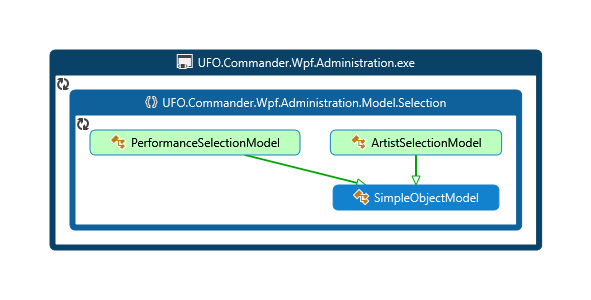
\includegraphics[scale=0.8]{\imagesRoot/simpleobjectmodel_map.PNG}
	\caption
	{Klasse für Controls mit Konverter}
\end{figure}
\ \\
Die beiden abgeleitet Klassen erweitern hierbei die Klasse \emph{SimpleObjectModel} um spezifische Attribute, die in dern Controls verwendet werden.

\newpage
\textbf{\emph{IConverter}}\\
Folgendes Klassendiagramm zeigt die Hierarchien der Klasse \emph{IConverter}.
\begin{figure}[h]
	\centering
	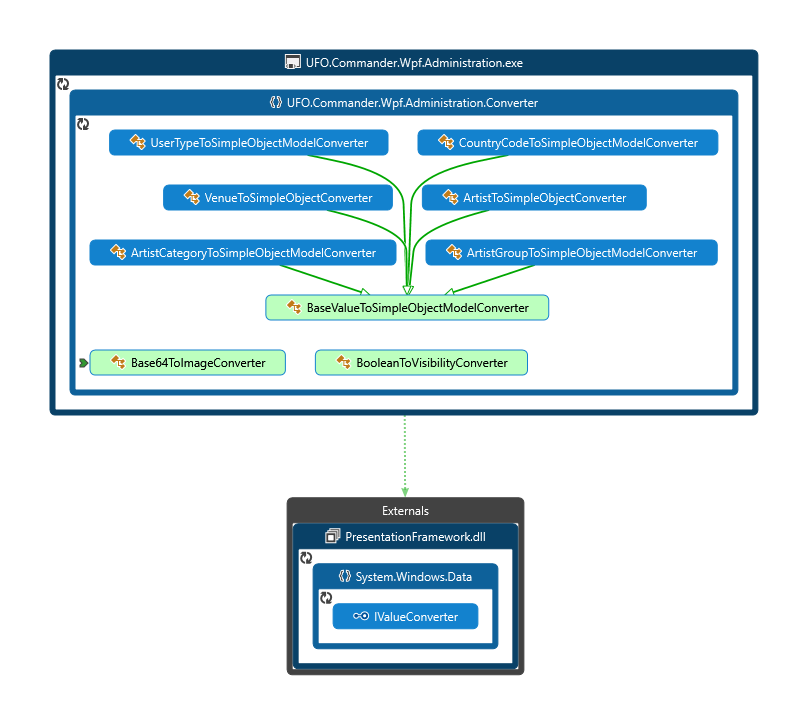
\includegraphics[scale=0.8]{\imagesRoot/iconverter_map.PNG}
	\caption
	{Konverter Hierarchie}
\end{figure}
\ \\
Die Klasse \emph{BaseValueToSimpleObjectConverter} stellt die Basisklasse aller Konverter dar, die Instanzen von \emph{SimpleObjectModel} konvertieren. In diese Klasse wurden alle gemeinsamen Funktionalitäten wie 
\begin{enumerate}
	\item\emph{Typprüfung}\\
	ES wird geprüft ob der Typ des übergebenen Value dem erwarteten Typ entspricht
	\item\emph{ConvertBack}\\
	Da hier nur Instanzen von \emph{SimpleObjectModel} konvertiert werden kann diese Methoden in einer Basisklasse implementiert werden, da hier nur auf den Property \emph{Data} zugegriffen wird.
\end{enumerate}
\ \\
Es wurden auch Konverter für die Visibility (true=Visibility.VISIBILE, false=Visibility.HIDDEN) und zum dekodieren von Base64 Strings in Image Instanzen eingeführt.

\newpage
\subsubsection{WPF Struktur}
Folgende Abbildung zeigt wie die Views innerhalb des Projektes strukturiert wurden.
\emph{IConverter}.
\begin{figure}[h]
	\centering
	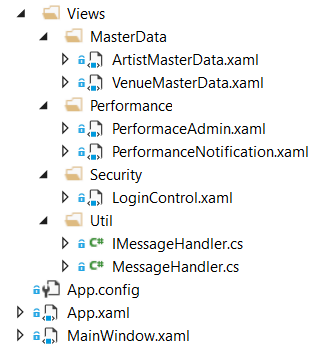
\includegraphics[scale=0.8]{\imagesRoot/viewfolderstructure.PNG}
	\caption
	{Verzeichnisstruktur der Views innerhalb des Projektes}
\end{figure}
\ \\
Bis auf die \emph{App.xaml} und \emph{MainView.xaml} wurden alle Views innerhalb eines Verzeichnis names \emph{Views} gebündelt wobei hierbei eine Trennung zwischen den einzelnen Typen der Views duchgeführt wurde.
\begin{enumerate}
	\item\emph{MasterData}\\
	Alle Views für dier Verwaltung der Stammdaten
	\item\emph{Performance}\\
	Alle Views für die Verwaltung des Festivalprogramms
	\item\emph{Security}\\
	Die Login-View
	\item\emph{Util}\\
	Utility Klassen um innerhalb von View-Models mit der View zu interagieren ohne Referenzen auf View Namespaces verwenden zu müssen.
\end{enumerate}
\ \\
Alle diese Views sind als UserControls implementiert worden und werden innerhalb von \emph{MainView.xaml} verwendet (außer PerformanceNotification.xaml), die diese UserControls in einem Tab-Control als DataTemplate für die verschiedene Typen der Tab-Models definiert.

\newpage
Folgende Abbildung zeigt die eingeführte Verzeichnisstruktur um die WPF-Ressourcen innerhalb diese Projektes zu strukturieren.
\begin{figure}[h]
	\centering
	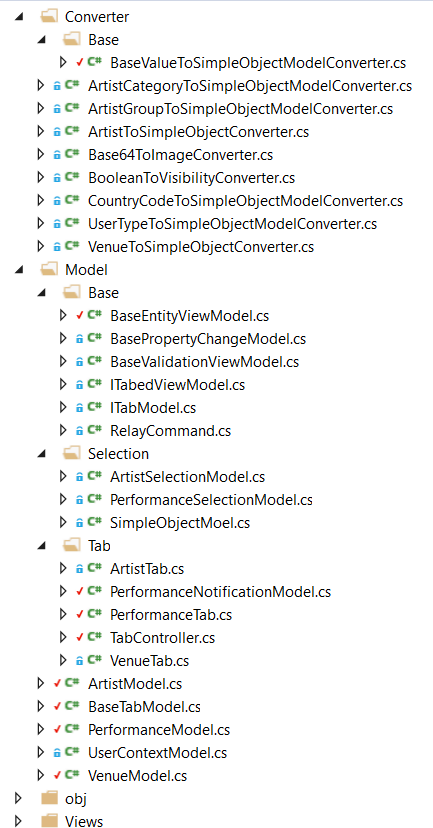
\includegraphics[scale=0.8]{\imagesRoot/wpffolderstrukture.PNG}
	\caption
	{Verzeichnisstruktur der WPF-Ressourcen}
\end{figure}
\ \\
Die jeweiligen Base-Verzeichisse beinhalten die eingeführten Basisklassen für den jeweiligen Kontext (z.B.: Converter, Models, ...).

\newpage
\subsubsection{Benutzerdokumentation}
Folgenden ist die Benutzerdokumentation der WPF-Anwendung \emph{Commander} angeführt.

\end{document}  